\documentclass[a4paper, 12pt]{article}
\usepackage[brazil]{babel}
\usepackage[a4paper, inner=2.5cm, outer=2.5cm, top=2.5cm, bottom=2.5cm]{geometry}
\usepackage{charter} % fonte utilizada no documento
                    %\usepackage[nf]{coelacanth}% fontes alternativas
                    %\usepackage[T1]{fontenc} % fontes alternativas
\usepackage[utf8]{inputenc} % indicação de caracteres especiais - contidos no pt
\usepackage{microtype} %server para formatação de espaçamento e indentação
\usepackage{graphicx} % pacote de formatação e inserção de figuras
\usepackage{fancyhdr} % pacote de formatação e inserção de cabeçalho e rodapé
\usepackage{float} % pacote de formatação de tabelas e figuras
\usepackage[style=abnt, sorting=ynt]{biblatex} % formatação e configuração das referências
\usepackage{csquotes}
\usepackage[singlespacing]{setspace} % pacote de formatação e inserção de figuras

\pagestyle{fancy} % estilo do cabeçalho e rodapé
\fancyhf{}
%\rhead{Livro LPP}
%\lhead{Edifícios Energeticamente Autosuficientes em Vitória}
\rfoot{Página \thepage}

%-------início do artigo-------%
\begin{document}
\title{Edifícios Comerciais Energeticamente Autosuficientes em Vitória}
\author{Anderson A. Fraga}
\maketitle

%\begin{abstract}
    \noindent O consumo de energia no uso de edificações vem crescendo gradativamente ao longo
    das últimas décadas, fruto do desenvolvimento industrial e da revolução tecnológica
    que vem acompanhando este movimento. A emissão de gases poluentes e a modificação 
    do clima são consequências desse cenário de desenvolvimento e consumo. Aliado a 
    esses fatores, as edificações contribuem para o agravamento  desse  cenário,  uma  
    vez  que  o  uso  destas  acarreta  em  impactos  negativos significativos ao meio 
    ambiente. Em contraponto, edificações energeticamente eficientes vêm se tornando 
    pré-requisito  para  o  planejamento  de  novos  ambientes  construídos,  
    modificando  a forma  como  a  comunidade  percebe  a  relação entre a edificação  
    e  o  consumo de  energia.  Este trabalho  tem  como  objetivo  estudar  o  
    potencial  de  aplicação  do  conceito Zero Energy  para edificações comerciais, 
    com o intuito de verificar a validade do método para o cenário construtivo 
    brasileiro adotando como estudo de caso  uma edificação  em Vitória (ES). 
    Metodologicamente, este  estudo  foi  desenvolvido  com  base  em  três  grandes  
    etapas,  onde  a  primeira  consistiu  em realizar  o  levantamento  das  
    edificações  dentro  de  um  recorte  territorial  pré-estabelecido, selecionar 
    as características construtivas e arquitetônicas mais frequentes entre elas e 
    construir modelos  representativos  do  cenário  observado;  a  segunda  consistiu  
    em  submeter  os  modelos representativos à simulações computacionais para avaliar 
    o desempenho energético, as possíveis formas  de  eficientização  e  de  produção  
    de  energia;  e  por  fim,  a  terceira  etapa,  na  qual  foi realizada  avaliação  
    dos  resultados  e  da  viabilidade  econômica  de  implantação  do  sistema  
    de produção de energia. Os resultados mostraram que as estratégias de implementação 
    de sistemas de condicionamento de ar, de equipamentos e iluminação mais eficientes 
    são muito importantes para  a  economia  de  energia.  É  perceptível  que  a  
    proposição  de  soluções  construtivas  e arquitetônicas  mais  eficientes  em  
    relação  ao  desempenho  energético  associado  a  técnicas  de obtenção  de  
    energia  podem  resultar  em  uma  edificação  com  o  balanço  energético  nulo  
    ou próximo ao nulo. Esses resultados indicam que a adoção desse conceito para novas 
    edificações é factível e cada vez mais acessível à comunidade.
    \paragraph{Palavras-chave:} zero energy buildings; balanço energético nulo; edifício de escritório 12 
\end{abstract}\pagebreak
\begin{onehalfspace}
\footnotesize
    \noindent A energia elétrica é um recurso essencial para o desenvolvimento econômico de 
    um país, para a qualidade de vida da população e para a manutenção do meio ambiente
    por meio de seu uso eficiente. A importância do uso racional e eficiente deste
    recurso torna imprescindível a conservação e redução do seu desperdício para a 
    sustentabilidade do ambiente em que se vive. Esta gestão eficiente do consumo de energia
    é essencial para reduzir o impacto energético de setores como o de edificações, 
    o qual consome cerca de 36 a 40\% da energia total final no mundo.\vspace*{0.3cm}
    
    \noindent Um exemplo da importância deste recurso e de seu uso devidamente planejado 
    pôde ser observado durante a crise brasileira. Ocorrida em 2001, esta crise provocou 
    mudanças no planejamento do fornecimento de energia elétrica, com o posterior 
    surgimento de medidas atenuantes às dificuldades de cunho ambiental e de 
    infraestrutura da época. Em seu ápice, no ano de 1999, o país passou pelo período 
    popularmente denominado “apagão”, o qual representou a falta de fornecimento 
    em 70\% do território nacional. O consumo de energia elétrica, entre os anos 
    de 1990 e 2000, sofreu aumento de 49\%, enquanto a capacidade instalada foi 
    expandida em 35\%, ocasionando o descompasso entre consumo e fornecimento 
    nesta época.\vspace*{0.3cm}

    \noindent Em contraponto à demanda e ineficiência energética, as edificações
    comerciais, em particular as de escritório, podem desempenhar funções estratégicas 
    como minimizar o uso energético e produzir eletricidade, aproximando ou tornando 
    zero a razão entre a produção e o consumo de energia. Estas edificações são 
    denominadas edificações com balanço energético nulo, 
    ou \textit{Zero Energy Buildings} – ZEB.\vspace*{0.3cm}

    \noindent Com a introdução de uma ZEB, a exploração de recursos renováveis complementares 
    como a energia solar, e a utilização de tecnologia solar fotovoltaica, surgem como 
    opção para minimizar as consequências negativas causadas por condições climáticas, 
    de infraestrutura e socioeconômicas adversas. A disponibilidade de recursos naturais 
    como a radiação solar recebida no Brasil, por exemplo, concentra grande capacidade de 
    geração de energia solar. Esta mesma quantidade de radiação está acima dos níveis de 
    países tradicionais na geração de energia fotovoltaica, o que ratifica a adoção deste 
    recurso como forma de reduzir o uso de fontes de energia fósseis.\vspace*{0.3cm}

    \noindent No âmbito estadual, o Espírito Santo vem apresentando redução na produção 
    de energia limpa quando comparado proporcionalmente ao consumo de fontes tradicionais. 
    Existe ainda a parcela de geração de energia elétrica oriunda de fontes não-renováveis 
    de energia, como usinas termelétricas, correspondendo a 65\% de toda a capacidade 
    instalada em operação do Espírito Santo, restando 35\% de fontes renováveis, composta 
    por usinas hidrelétricas, com participação de 34\%, e geradores de energia solar 
    fotovoltaica, com 1\%.\vspace*{0.3cm}

    \noindent Além do baixo aproveitamento de energias provenientes de fontes 
    renováveis, o estado ainda conta com edificação com baixo desempenho termoenergético, 
    principalmente edificações comerciais. Estas, mesmo após legislações sobre metas de 
    desempenho energético publicadas após 2003, não atendem boa parte dos critérios 
    definidos, muito menos adotam materiais e componentes com a eficiência necessária 
    para desenvolver um estado de uso eficiente de energia elétrica.\vspace*{0.3cm}

    \noindent Desta forma, considerando as características do ambiente construído no 
    âmbito da Região Metropolitana da Grande Vitória e brasileiro, uma questão foi 
    levantada: é possível desenvolver edificações cujos valores de demanda e produção de 
    energia elétrica resultem em nulo ou quase nulo em Vitória? Assim, o objetivo 
    principal desta pesquisa foi avaliar a aplicabilidade do conceito \textit{Zero Energy}
    em edificações comerciais, especificamente de escritório, com o intuito de 
    verificar a validade do método para o cenário construtivo brasileiro, utilizando 
    como recorte territorial e cenário urbano para o estudo a cidade de 
    Vitória (ES).\vspace*{0.3cm}

    \noindent Como ponto de partida, define-se que um edifício \textit{Zero Energy} – ZEB, 
    ou em português, balanço energético nulo, é uma edificação energeticamente eficiente 
    onde, considerada a fonte energética, a energia elétrica fornecida pela concessionária 
    é anualmente menor ou igual à quantidade de energia renovável exportada pela 
    edificação para a rede.\vspace*{0.3cm}

    \noindent Uma outra definição importante iniciada na Europa foi proposta para 
    edificações \textit{Near Net Zero Energy}, nZEB, e em português, próximo ao 
    balanço energético nulo, se apoia na premissa do aproveitamento máximo 
    de recursos para produção de energia, implementando mecanismos à edificação de 
    forma que este aproveitamento aconteça, e a utilização à nível ótimo da energia 
    primária, para um consumo maior que 0 kWh/m² ao ano.\vspace*{0.3cm}

    \noindent Ainda sobre a eficiência energética no ambiente construído, estudos desenvolvidos pela \textit{United Nations Enviroment Programme}
    apontam que 103 países definiram a eficiência energética e uso de energias 
    renováveis como parte importante do seu planejamento estratégico, e destes, 
    79 são países emergentes e em desenvolvimento. Constata-se, ainda, que o 
    consumo de energia poderia ter sido 12\% maior em 2017 caso as políticas 
    públicas mencionadas anteriormente não tivessem sido implementadas desde o ano 2000.\vspace*{0.3cm}

    \noindent Após a definição dos conceitos, o trabalho foi desenvolvido com base em três 
    grandes etapas, onde a primeira consistiu em realizar o levantamento das edificações 
    dentro de um recorte territorial pré-estabelecido, selecionar as características 
    construtivas e arquitetônicas mais frequentes entre elas e construir modelos 
    representativos do cenário observado; a segunda consistiu em submeter os modelos
    representativos à simulações computacionais para avaliar o desempenho energético, 
    as possíveis formas de eficientização e de produção de energia; e por fim, a 
    terceira etapa, na qual foi realizada avaliação dos resultados e da viabilidade 
    econômica de implantação do sistema de produção de energia, como representado 
    na Figura 1.\vspace*{0.3cm}
    \begin{figure}[H]
        \centering
        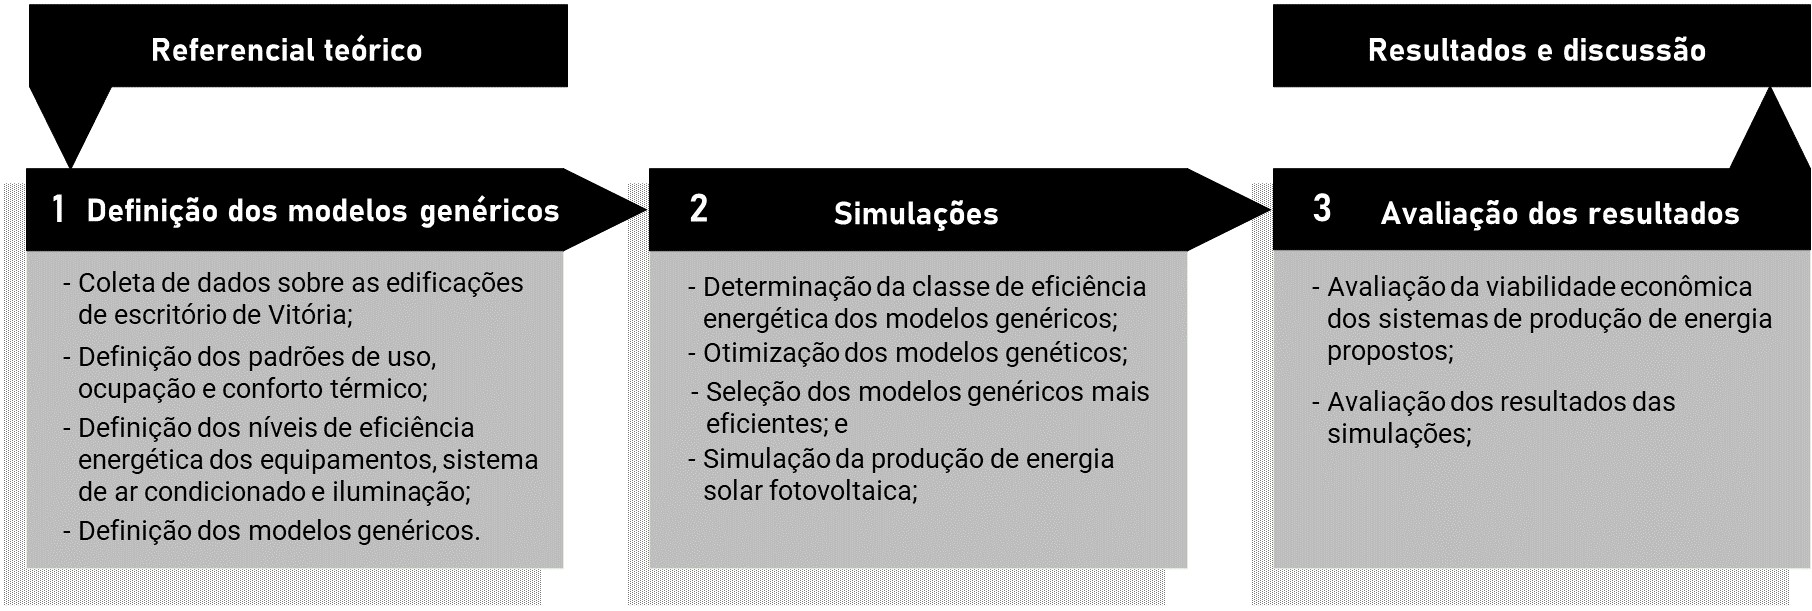
\includegraphics[width=0.9\textwidth]{figures/0_Fluxogramas1 (2).jpg}
        \begin{flushleft}
            \small Figura 1 - Fluxograma da avaliação da edificação.
        \end{flushleft}
    \end{figure}
    \noindent Após a conclusão do levantamento, as edificações selecionadas foram resumidas às
    características mais frenquentes entre elas e, assim, traduzidas em um modelo computacional
    que compusesse um retrato das edificações comerciais de escritório da cidade de Vitória.
    Essas características foram divididas entre dois modelos com quantidades de pavimento-tipo
    que representassem edificações com menos pavimentos, com 8, e mais pavimentos, com 19, como
    mostra a Figura 2.

    \noindent Os edifícios selecionados foram resumidos às características mais frequentes 
    entre elas e, assim, traduzidas em um modelo computacional que compusesse um retrato 
    das edificações comerciais de escritório da cidade de Vitória. Essas características 
    foram divididas em dois modelos com quantidades de pavimento-tipo que representassem 
    edificações com menos pavimentos, com 8, e mais pavimentos, com 19, como mostra a 
    Figura 2. Além do número de pavimentos, elas conformam dois pavimentos-garagem, 
    um pavimento térreo composto por lojas e cada pavimento-tipo contém 9 salas 
    comerciais e 1 área com circulações verticais e horizontais.\vspace*{0.3cm}
    \begin{figure}[H]
        \centering
        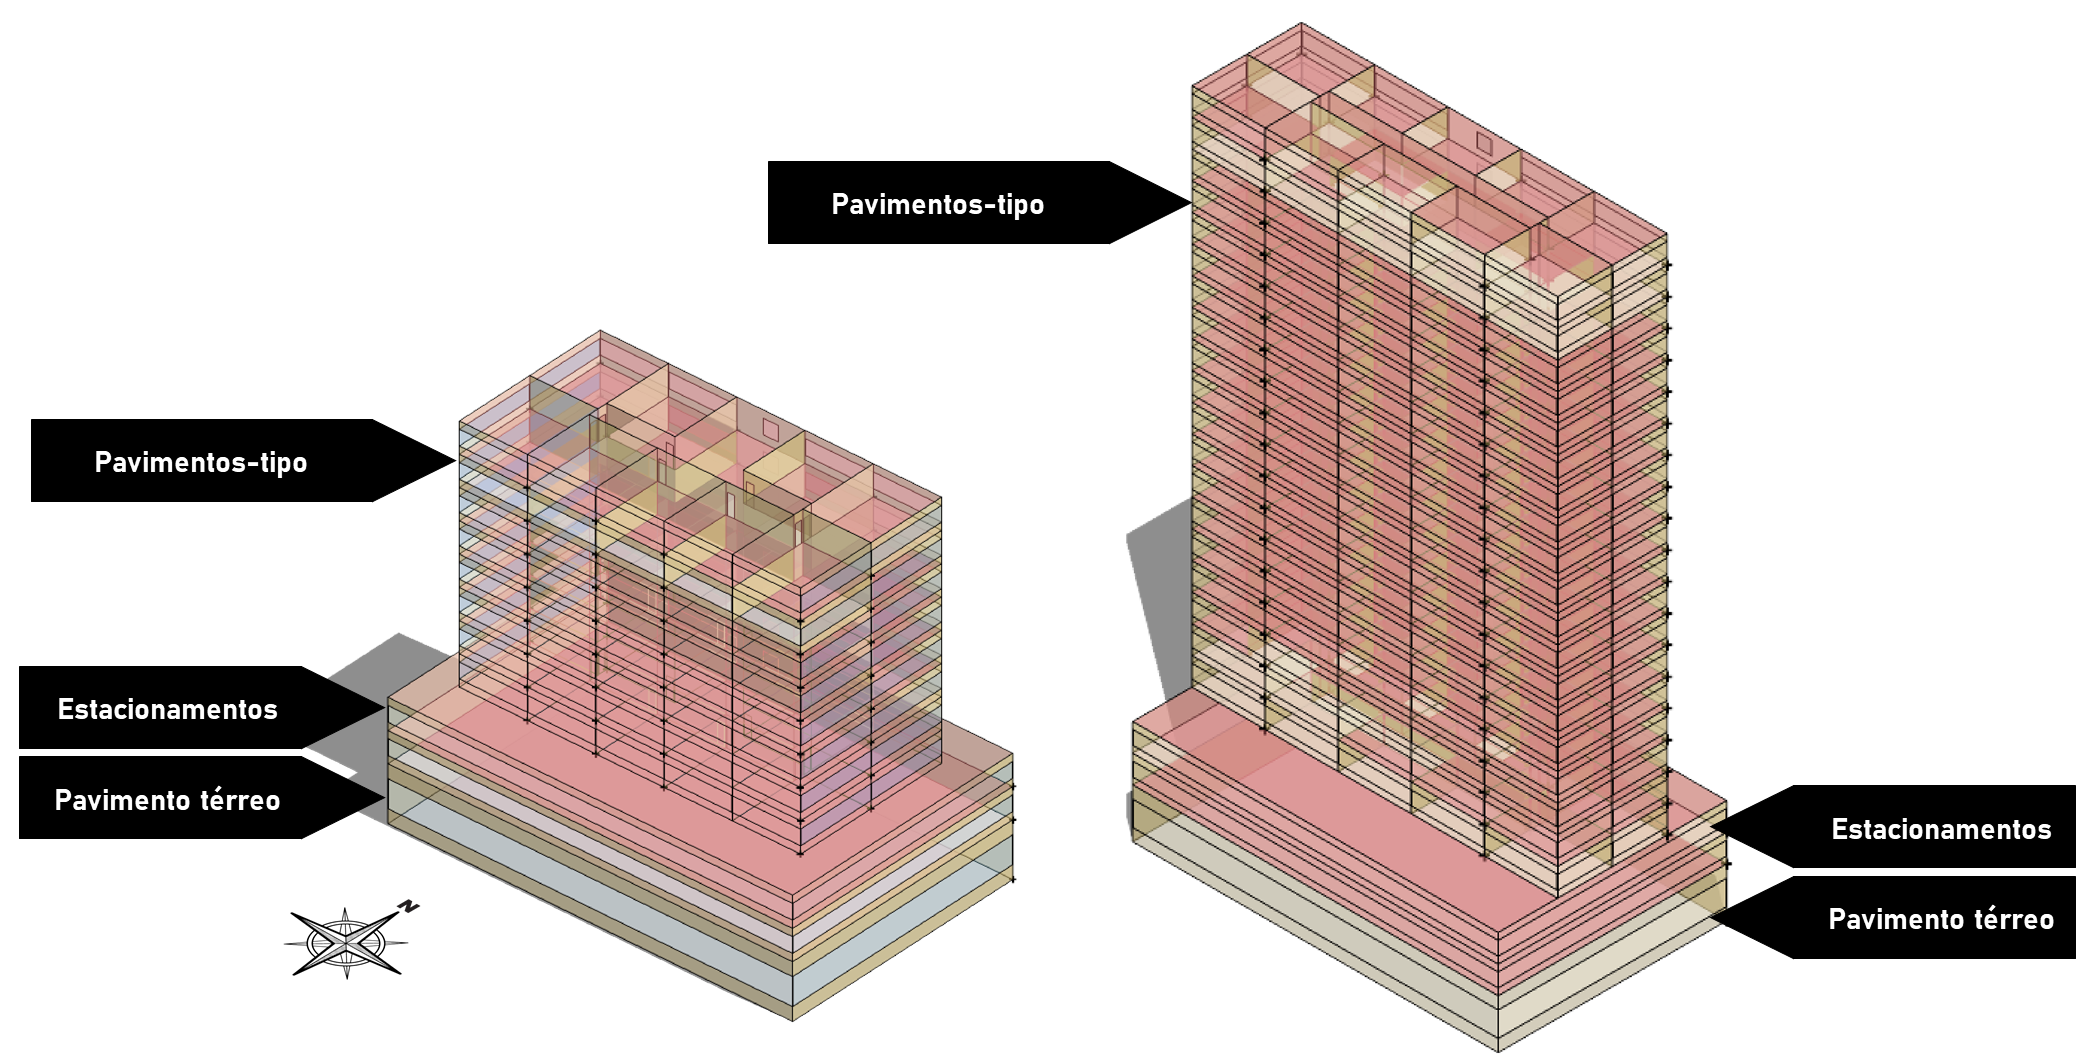
\includegraphics[width=1\textwidth]{figures/fig11_8-19-2pav.png}
        \begin{flushleft}
            \small Figura 2 - Modelos computacionais de 8 pav. e 19 pav.
        \end{flushleft}
    \end{figure}
    \noindent Com a conclusão da etapa de modelagem computacional, representando o estado de desempenho
    energético das edificações locais, foram propostas melhorias à arquitetura e aos equipamentos
    identificados, assim como melhorias para o sistemas de condicionamento de ar, principal
    responsável pelo consumo de energia. Para contrapor o consumo de energia, aumentar a
    eficiência do modelo e utilizar o conceito de edificação \textit{Zero Energy}, foi proposto
    um sistema de produção de energia solar por meio de painéis fotovoltaicos, como exemplificado
    na Figura 3.
    \begin{figure}[H]
        \centering
        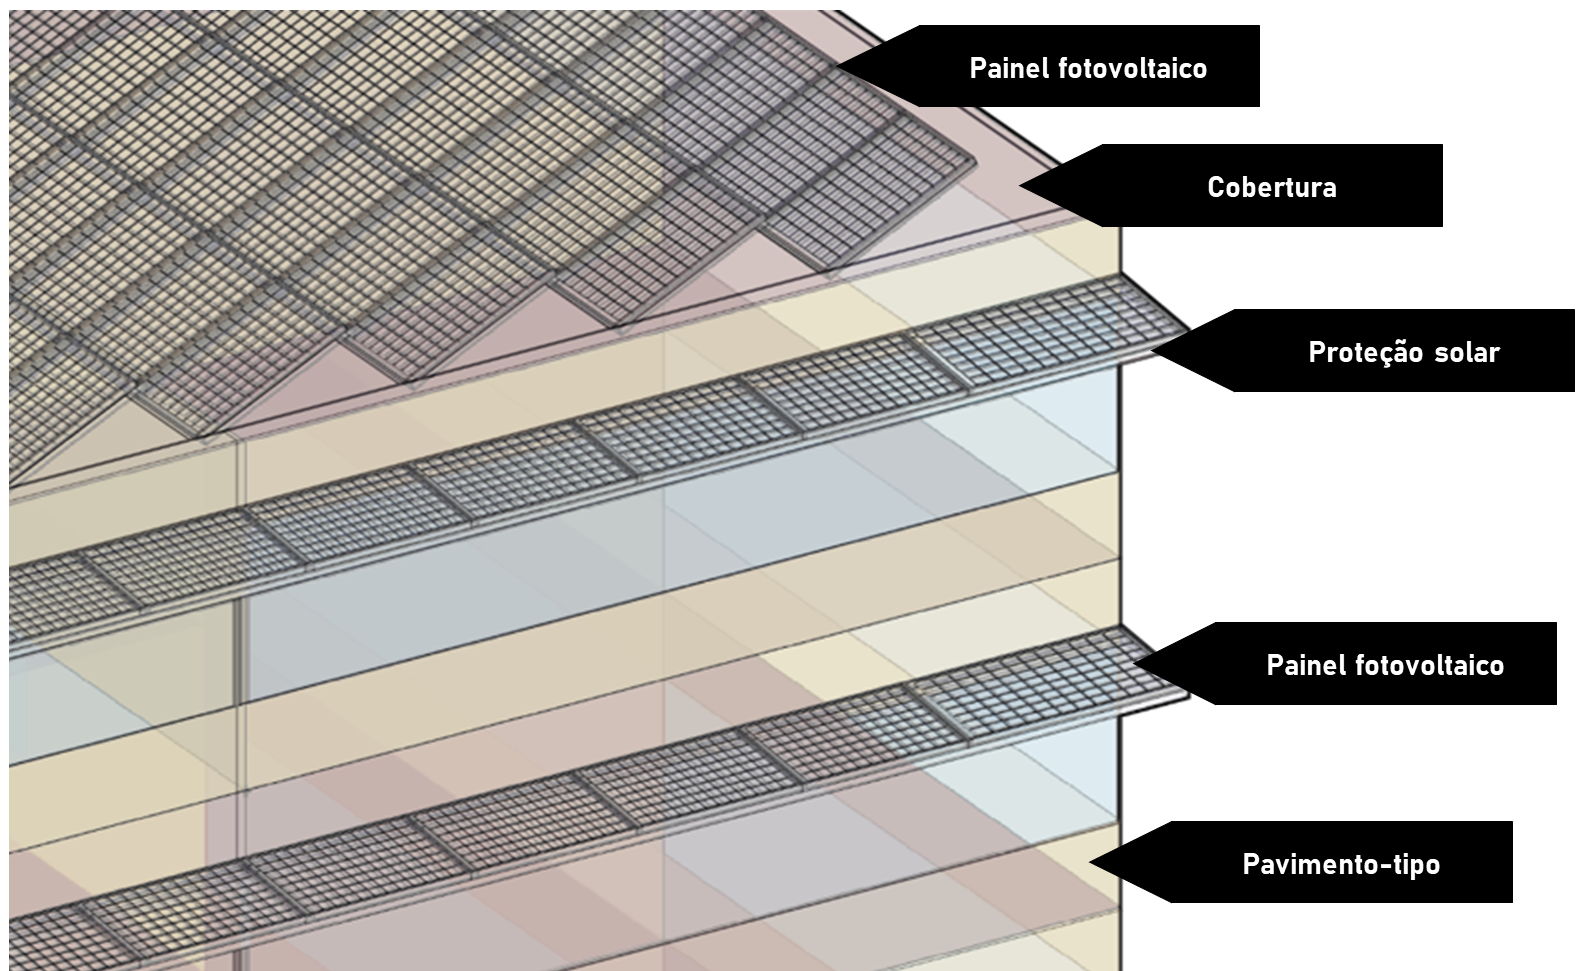
\includegraphics[width=0.85\textwidth]{figures/paineis pv.png}
        \begin{flushleft}
            \small Figura 3 - Sistema de produção de energia fotovoltaica.
        \end{flushleft}
    \end{figure}
    \noindent A verificação da validade das modificações propostas para melhoria de 
    desempenho do modelo foi feita por meio de simulações computacionais. Estas simulações
    tiveram a funçao de revelear, de uma forma detalhada, o impacto das modificações 
    arquitetônicas e de desempenho termoenergético dos modelos. Assim, esta etapa de 
    de simulação foi composta por cenários onde as modificações foram implementadas 
    de forma sequencial e incremental, ou seja, no primeiro cenário foi 
    modificada a composição dos vidros, de um menos eficiente para o mais eficiente 
    no mercado. No segundo cenário foi mantida a melhor opção de vidro para o modelo, e,
    adicionalmente, foram modificadas as aberturas dos modelos, e assim sucessivamente.
    Estes cenários foram agrupados em blocos de simulação, representados de B1 a B10, a fim
    de facilitar a identificação das modificações propostas e plotagem dos resultados em 
    gráfico.\vspace*{0.3cm}

    \noindent Os resultados mostraram que as estratégias de implementação de sistemas
    de condicionamento de ar, de equipamentos e iluminação mais eficientes são muito importantes
    para a economia de energia. É perceptível que a proposição de soluções construtivas e
    arquitetônicas mais eficientes em relação ao desempenho energético associado a técnicas de
    obtenção de energia podem resultar em uma edificação com o balanço energético nulo ou
    próximo ao nulo. Esses resultados indicam que a adoção desse conceito para novas edificações é
    factível e cada vez mais acessível à comunidade.\vspace*{0.3cm}

    \noindent Dentre as observações feitas sobre os resultados alcançados, e analisando 
    mais atentamente os resultados dos blocos de simulação, percebe-se que a reta azul de 
    média é mais acentuada no Gráfico 1, representativo do consumo anual final de energia 
    elétrica do modelo de 8 pavimentos, do que no Gráfico 2, representando o consumo 
    energético do modelo de 19 pavimentos. Esta diferença sugere que as modificações 
    atribuídas em ambos os modelos são mais eficazes no modelo com menos pavimentos do que 
    no modelo maior.\vspace*{0.3cm}
    \begin{figure}[H]
        \centering
        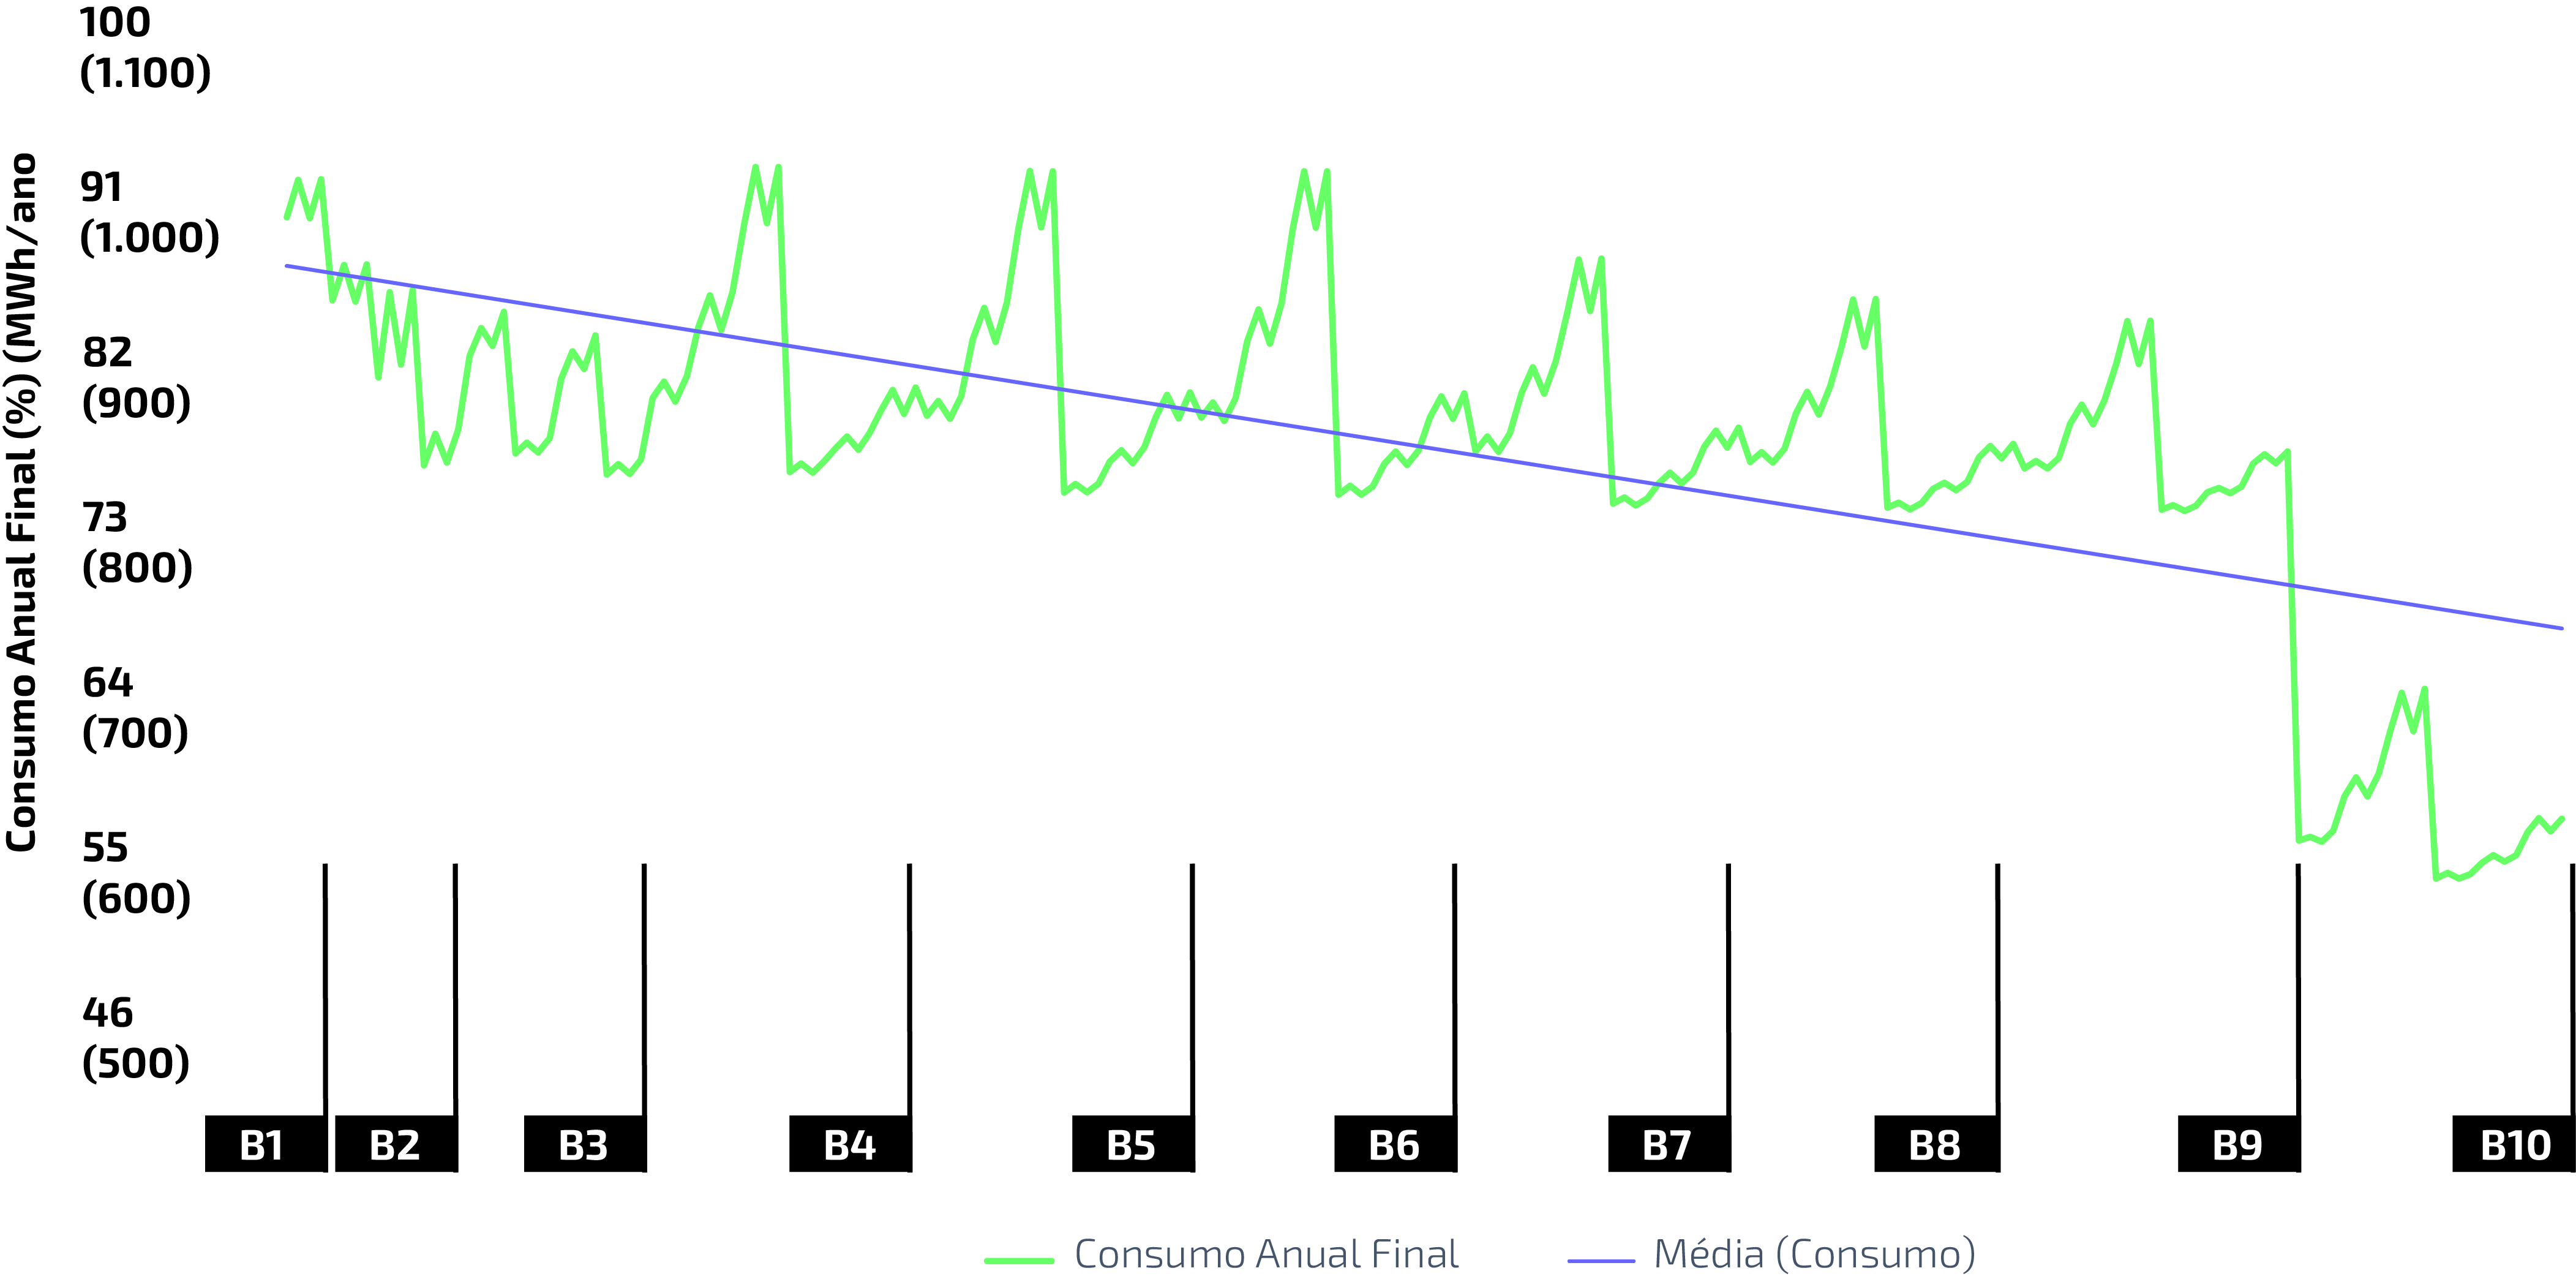
\includegraphics[width=1\textwidth]{figures/grafico-8pav.png}
        \begin{flushleft}
            \small Gráfico 1 - Curva de Consumo Anual Final de energia elétrica do modelo de 8 pavimentos.
        \end{flushleft}
    \end{figure}
    \noindent Observa-se, também, que o desempenho da edificação de 19 pavimentos aumenta 
    após a inserção de um sistema de ar condicionado mais eficiente do que os modelos 
    observados nos edifícios da cidade. Este aumento de desempenho pode ser observado no 
    comportamento da curva entre B1 e B3, no Gráfico 2. Já para o modelo com tipologia de 
    8 pavimentos, a mudança de um vidro de baixo para alto desempenho termoenergético resultou 
    em uma queda significativa de consumo de energia, como apresentado no Gráfico 1, curva 
    entre B9 e B10.\vspace*{0.3cm}
    \begin{figure}[H]
        \centering
        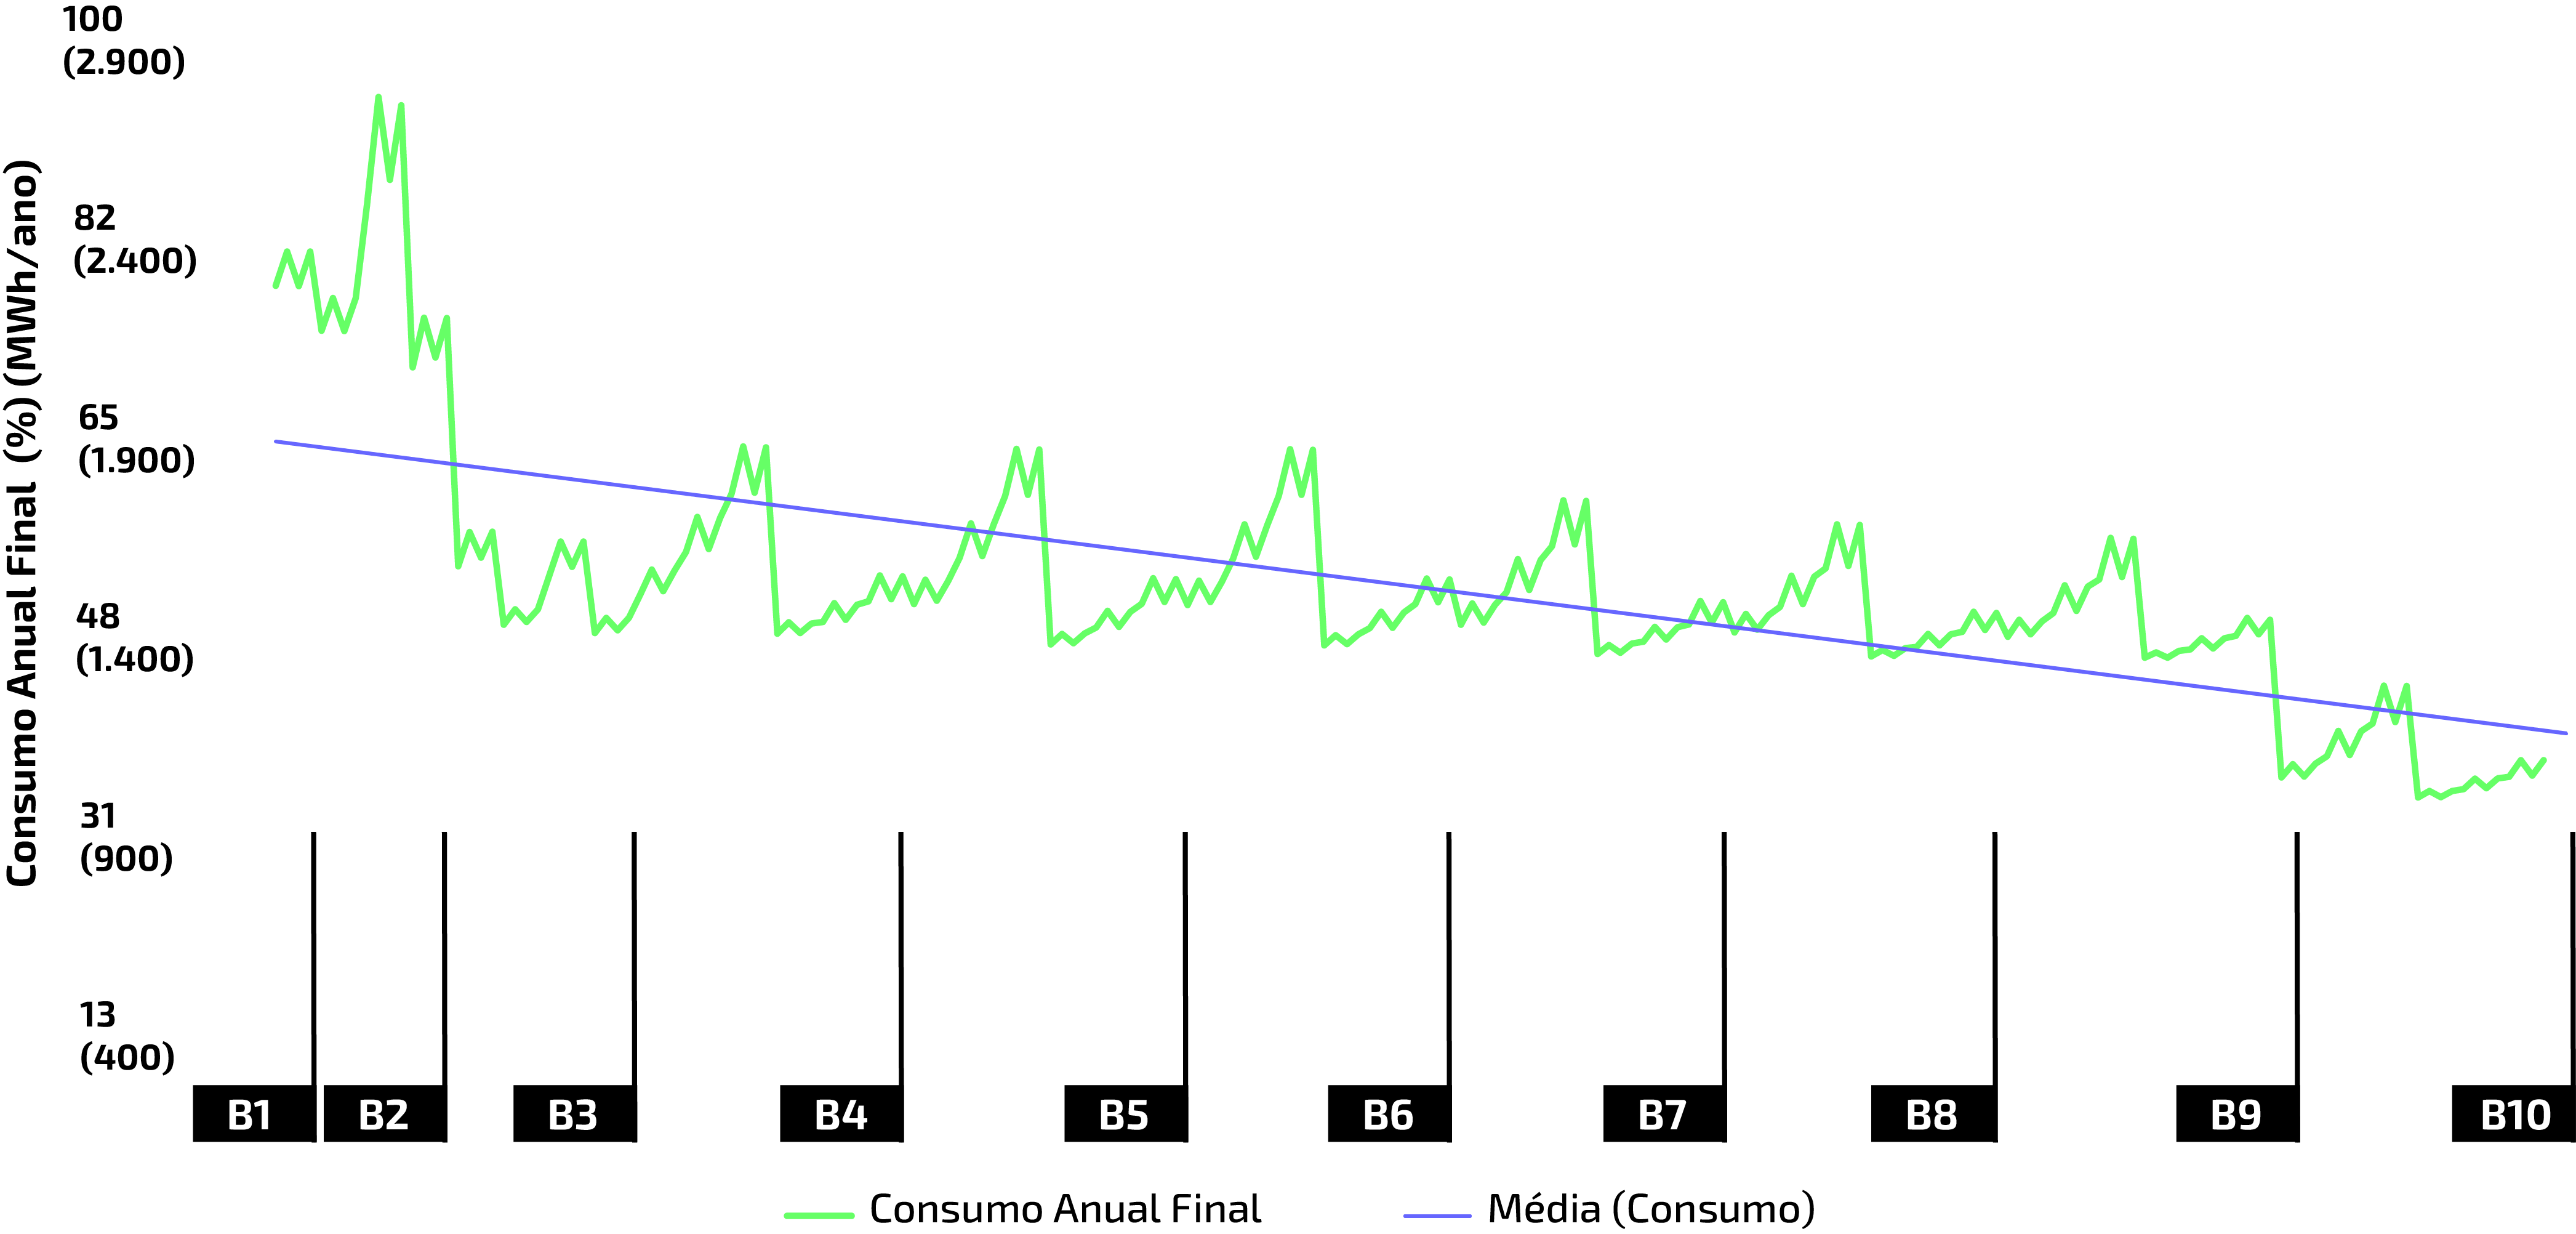
\includegraphics[width=1\textwidth]{figures/grafico-19pav.png}
        \begin{flushleft}
            \small Gráfico 2 - Curva de Consumo Anual Final de energia elétrica do modelo de 19 pavimentos.
        \end{flushleft}
    \end{figure}
    \noindent As modificações arquitetônicas propostas para os modelos resultaram em pouco 
    impacto quando os resultados são analisados de forma individual. Entretendo, quando 
    estes mesmos resultados são analisados de forma global, é perceptível a importância 
    dessas alterações, dada a gradativa redução de energia com mudanças com relativo baixo 
    custo de implementação.\vspace*{0.3cm}

    \noindent Sendo assim, concluiu-se que o potencial de produção de energia solar, 
    dada a particularidade do desenho urbano da cidade e da grande presença de edificações 
    com poucos pavimentos, favorece a implementação do conceito \textit{Zero Energy} para 
    as edificações comerciais. Como exemplo imediato da importância deste estudo, medidas 
    no sentido de estudar a validade do conceito foram adotadas recentemente pelo Governo 
    Federal, por meio de uma chamada pública para propostas de edificações que utilizassem 
    o conceito Zero Energy como diretriz projetual, com o intuito de tornar válida e 
    popularizar a iniciativa de construções energeticamente eficientes.
\end{onehalfspace}


%\bibliography{ref.bib}
%\printbibliography

\end{document}